\documentclass[border=10pt]{standalone}

\usepackage{tikz}
\usepackage{tikzsymbols}
\usetikzlibrary{calc,patterns,shapes.geometric}

\def\centerarc[#1](#2)(#3:#4:#5){\draw[#1] ($(#2)+({#5*cos(#3)},{#5*sin(#3)})$) arc (#3:#4:#5);}

\begin{document}
	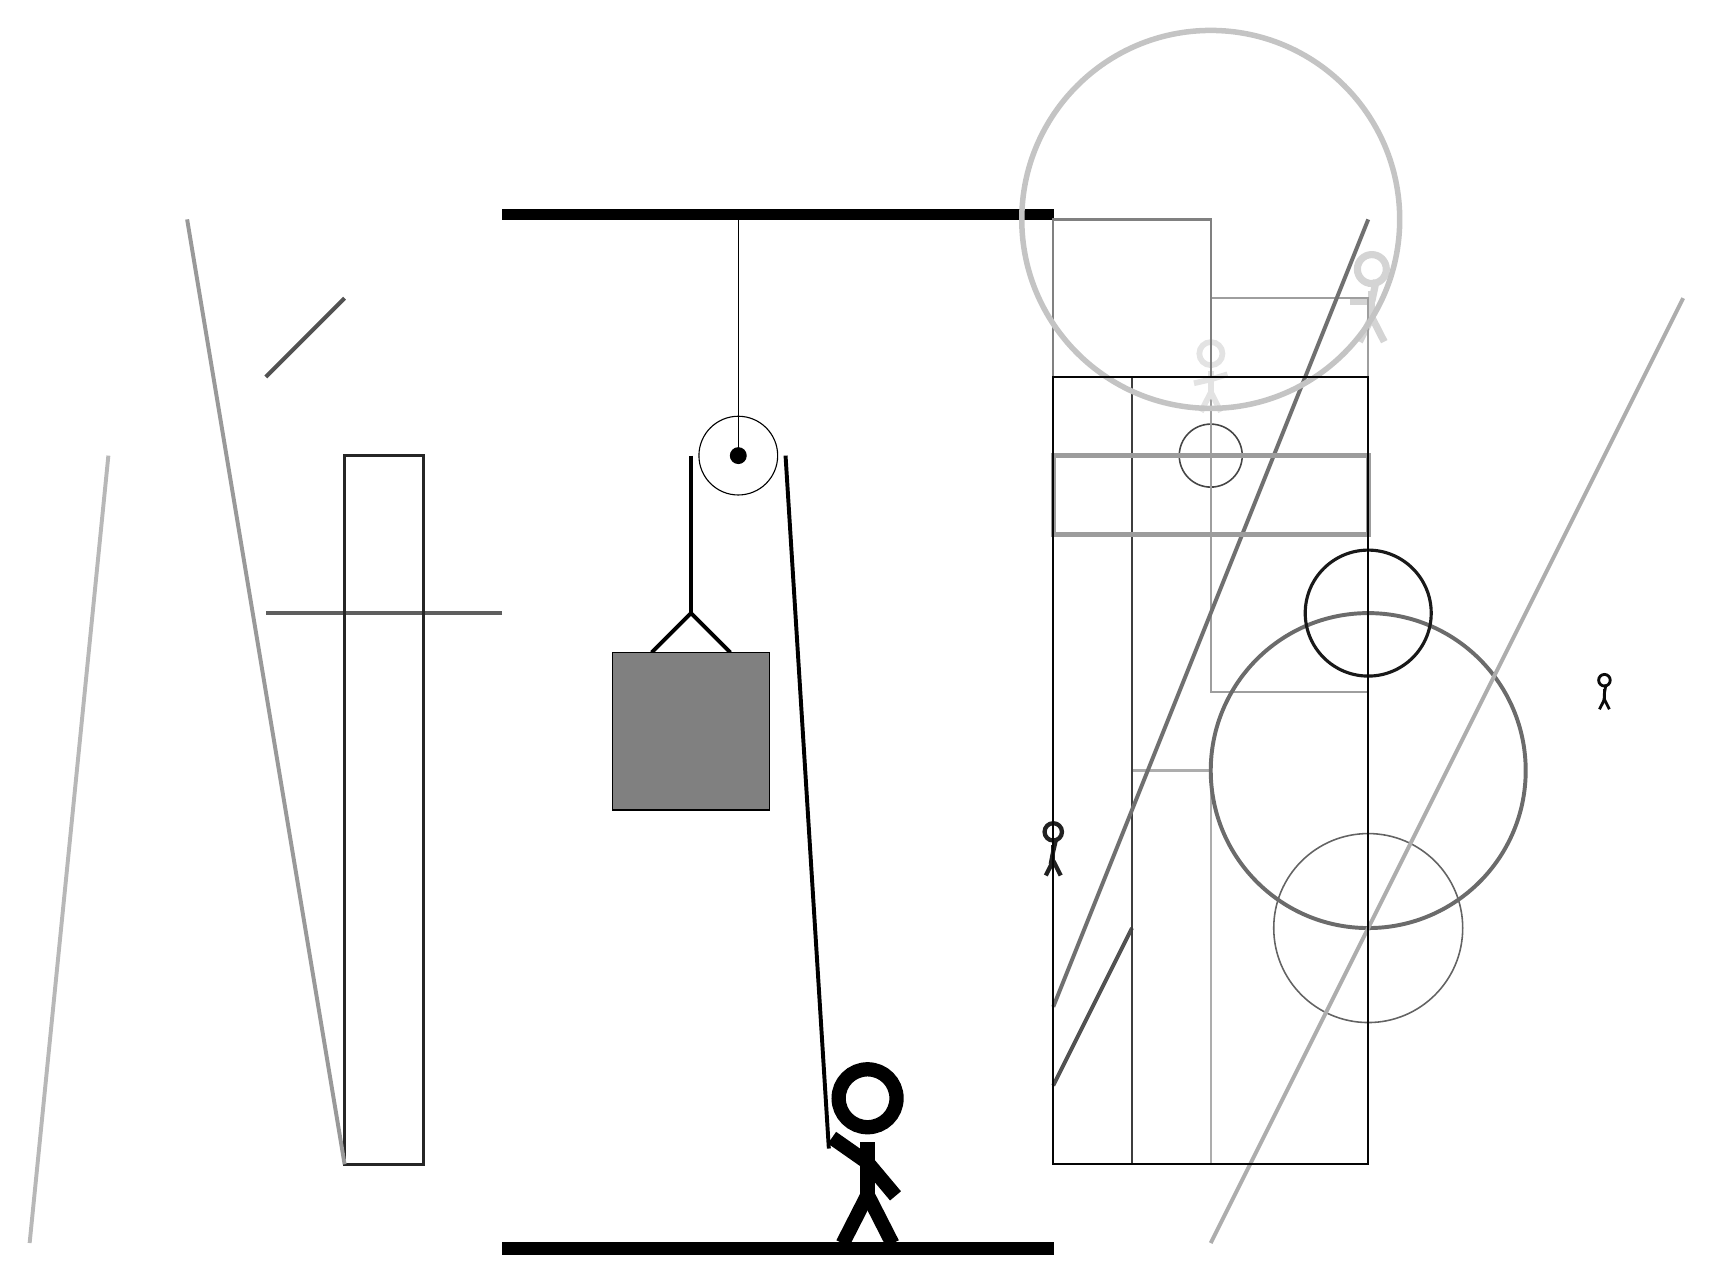
\begin{tikzpicture}
		%%%%% START %%%%%
		
		\draw[fill=black] (-2, 10) rectangle (5, 10.125);
		
		\draw (1, 7) circle (0.5);
		\draw[fill=black] (1, 7) circle (0.1);
		\draw (1, 10) -- (1, 7);
		
		\draw[line width=0.5mm] (-0.1, 4.5) -- (0.4, 5.0) -- (0.9, 4.5);
		\draw[fill=black!50] (-0.6, 4.5) rectangle (1.4, 2.5);
		
		\draw[line width=0.5mm] (0.4, 7) -- (0.4, 5.0);
		\centerarc[line width=0.5mm](1, 7)(0:180:0.6);
		\draw[line width=0.5mm](1.6, 7) -- (2.15, -1.8);
		
		\node at (2.6, -1.9) {\Strichmaxerl[10][-35][-50]};
		
		\draw[line width=0.3mm, color=black!32] (6, 3) rectangle (7, -2);
		
		\draw[line width=0.5mm, color=black!68](6, 1) -- (5, -1);
		\node[line width=0.6mm, color=black!96] at (12, 4) {\Strichmaxerl[2][87][80]};
		\node[line width=0.2mm, color=black!17] at (9, 9) {\Strichmaxerl[5][0][78]};
		
		\draw[line width=0.5mm, color=black!63](-2, 5) -- (-5, 5);
		\draw[line width=0.4mm, color=black!85] (-3, 7) rectangle (-4, -2);
		\draw[line width=0.5mm, color=black!28](-7, 7) -- (-8, -3);
		
		\draw[line width=0.2mm, color=black!76] (6, -2) rectangle (6, 8);
		\draw [line width=0.2mm, color=black!73](7, 7) circle (0.4);
		\draw[line width=0.3mm, color=black!38] (7, 9) rectangle (9, 4);
		\draw[line width=0.5mm, color=black!56](5, 0) -- (9, 10);
		
		\draw [line width=0.2mm, color=black!61](9, 1) circle (1.2);
		\draw[line width=0.6mm, color=black!39] (5, 6) rectangle (9, 7);
		\draw[line width=0.5mm, color=black!68](-4, 9) -- (-5, 8);
		\node[line width=0.5mm, color=black!87] at (5, 2) {\Strichmaxerl[3][79][77]};
		\draw [line width=0.5mm, color=black!58](9, 3) circle (2.0);
		
		\draw[line width=0.5mm, color=black!32](7, -3) -- (13, 9);
		
		\node[line width=0.2mm, color=black!11] at (7, 8) {\Strichmaxerl[4][13][17]};
		\draw [line width=0.4mm, color=black!90](9, 5) circle (0.8);
		
		\draw[line width=0.5mm, color=black!40](-6, 10) -- (-4, -2);
		\draw[line width=0.3mm, color=black!50] (5, 10) rectangle (7, 8);
		
		\draw [line width=0.7mm, color=black!23](7, 10) circle (2.4);
		\draw[line width=0.3mm, color=black!98] (5, 8) rectangle (9, -2);
		
		\draw[fill=black] (-2, -3) rectangle (5, -3.15);
		
		%%%%% END %%%%%
	\end{tikzpicture}
\end{document}